% Crisis Zones — research paper
% Build: pdflatex geoint-crisis-zones.tex (twice). Figures in figures/.

\documentclass[11pt,a4paper]{article}
\usepackage[utf8]{inputenc}
\usepackage[T1]{fontenc}
\usepackage{lmodern}
\usepackage{microtype}
\usepackage[margin=2.5cm]{geometry}
\usepackage{booktabs}
\usepackage{array}
\usepackage{parskip}
\usepackage{enumitem}
\usepackage{graphicx}
\usepackage{subcaption}
\usepackage{xcolor}
\usepackage{tikz}
\usetikzlibrary{arrows.meta,positioning,fit,backgrounds}
\usepackage{amsmath}
\usepackage[hidelinks]{hyperref}
\usepackage{url}

\linespread{1.08}
\graphicspath{{figures/}}
\setlist{itemsep=2pt,topsep=4pt}

\newcommand{\appname}{Crisis Zones}
\newcommand{\repourl}{https://github.com/suadarzimanli/geoint-crisis-zones}
\newcommand{\archivedoi}{(\href{https://doi.org/10.5281/zenodo.24417729}{doi:10.5281/zenodo.24417729})}

\title{Mapping and Forecasting Protest and Political Violence\\ in Poland:
       A GEOINT Web Application and an Evaluation\\ of County-Level Event Forecasts}
\author{Suad Arzimanli\\[2pt]
        \small University of \L{}ód\'{z}, Faculty of Mathematics and Computer Science, Poland\\
        \small \texttt{suad.arzimanli@gmail.com}}
\date{}

\begin{document}
\maketitle

\begin{abstract}
Event datasets such as ACLED make it possible to follow protest and political violence at the level of individual, geocoded events. Analysts and civil-protection staff need to move quickly from a national overview to the record of a single event, and they increasingly see short-term forecasts next to the map. This paper presents \appname{}, an open-source web application for the 7{,}794 ACLED events recorded in Poland from January 2020 to December 2024, and evaluates the next-month forecast it shows for each of the country's 341 counties.

The design follows the sequence \emph{overview, filter, details on demand}. Because ACLED geocodes most events to a town or district centre, 95.5\% of events share their exact coordinates with at least one other event (a single point in Warsaw holds 1{,}132), so the interface treats places, not points, as the unit of selection. The forecast is a three-month moving average whose inputs are displayed beside every value.

The evaluation compares eight methods, from always predicting zero to a Random Forest, on 4{,}092 held-out county-months, with every method predicting each month only from earlier months. Among the methods that predict activity at all, accuracy differences are small: the Random Forest has the lowest root-mean-square error (1.35 events per county-month against 1.43 for the moving average), but a county-level bootstrap interval for the difference includes zero, and the moving average is more accurate on a six-month window. The ranking depends more on the evaluation design than on the method: when months without events are dropped and the methods draw on different information, the Random Forest appears 30\% more accurate than the moving average; when all methods see the same history, their errors on months with events are equal to two decimals. The results support a transparent baseline as the displayed forecast and argue for reporting forecast accuracy together with the protocol that produced it.

\medskip
\noindent\textbf{Keywords:} geospatial intelligence; GEOINT; ACLED; conflict event data; protest; web GIS; count forecasting; forecast evaluation; Poland.

\smallskip
\noindent\textbf{Disclaimer.} Independent academic project, not affiliated with ACLED. The application displays reported events; its forecasts are not risk assessments.
\end{abstract}

%======================================================================
\section{Introduction}
\label{sec:intro}

When unrest spreads, the first questions are spatial: where is it happening, how concentrated is it, and where is it likely to continue? Geospatial intelligence (GEOINT) is the practice of answering such questions by integrating location-linked information \cite{nga2018}. Imagery dominates the public picture of GEOINT, but event datasets are equally important. They record what happened, when, who was involved and where, already tied to coordinates. The Armed Conflict Location \& Event Data project (ACLED) curates political violence and demonstration events worldwide with consistent categories and geocoding \cite{raleigh2010,acled2024}. In a country such as Poland, where the record is dominated by demonstrations rather than armed conflict, such data serve civil protection, public-order planning and policy analysis as much as security analysis.

Applications built on event data commonly import a table, plot points and add filters. Two gaps remain. The first is \emph{reading the evidence}: a national map of thousands of markers shows density but makes it hard to reach the record behind a point, especially on a phone, and especially when many events share one location. The second is \emph{forecast accountability}: once a forecast panel is added, its numbers look authoritative whether or not anyone has scored them, and the score itself depends on choices---which months are tested, whether months without events are counted, what information each method may use---that are rarely reported \cite{tashman2000,kapoor2023}.

\subsection{Research questions}

\begin{description}[leftmargin=2.6em,style=nextline]
  \item[RQ1] How can an event-level dataset be presented so that a user can move from a national overview to the record of an individual event, on desktop and phone, while every forecast stays traceable to its inputs?
  \item[RQ2] What spatial and temporal structure does ACLED's record for Poland show, and what does that structure imply for forecasting at the county level?
  \item[RQ3] How accurately do simple and learned methods predict next-month event counts per county when all methods use the same information?
  \item[RQ4] How much do evaluation choices---the treatment of months without events, the information available to each method, and the error metric---change the ranking of methods?
\end{description}

RQ1 is a design question, answered by an implemented application. RQ2--RQ4 are empirical and are answered with the event data and a forecast evaluation.

\subsection{Contributions}

\begin{enumerate}
  \item \textbf{\appname{}}, an open-source web application (ASP.NET Core, Google Maps, Chart.js) for exploring ACLED events in Poland, with filters, linked charts, place-level event browsing and a county forecast panel that shows the months behind every value and the method's measured accuracy (\S\ref{sec:design}).
  \item A \textbf{description of the Polish event record} as a forecasting problem: sparse, spatially concentrated and shaped by a few national protest waves (\S\ref{sec:data}, \S\ref{sec:res-patterns}).
  \item A \textbf{forecast evaluation} of eight methods with a rolling one-step-ahead protocol, three test windows, several metrics and county-level bootstrap intervals (\S\ref{sec:eval}, \S\ref{sec:res-accuracy}).
  \item A \textbf{demonstration of protocol sensitivity}: the same methods ranked under two evaluation designs, showing how an apparent 30\% advantage of a learned model arises from the design rather than the model (\S\ref{sec:res-protocol}).
\end{enumerate}

The code, the evaluation and the aggregated data are public \cite{repo}. Raw ACLED records are not redistributed (\S\ref{sec:data-licence}).

%======================================================================
\section{Background}
\label{sec:background}

\subsection{GEOINT and event data}

GEOINT doctrine describes the integration of imagery, geospatial information and activity data to support decisions \cite{nga2018}. For protest-dominated contexts the operational question is rarely the movement of armed forces; it is early awareness of where demonstrations concentrate, which kinds of events occur, and whether activity is rising. Event datasets answer that question more directly than imagery. Interactive maps add value by making concentration visible, but only if users can move from the overview to the evidence: Shneiderman's information-seeking mantra---\emph{overview first, zoom and filter, then details on demand}---remains a sound organising principle for such interfaces \cite{shneiderman1996}.

\subsection{ACLED and reporting bias}

ACLED records each event with its date, disorder type, event type and sub-type, actors, interaction code, fatalities, administrative units, coordinates with a precision code, sources and a short narrative note \cite{raleigh2010,acled2024}. Events are coded from media, local partners and other sources, so the record reflects what is \emph{reported}. Reporting is denser in cities and where media and civil society are active \cite{weidmann2016}, and coverage decisions and coding rules shape the patterns that a dataset shows \cite{raleigh2023}. Any map or forecast built on such data inherits these properties.

\subsection{Forecasting conflict and protest}

Political-violence forecasting has moved from country-year models towards sub-national, monthly forecasts, as in the ViEWS early-warning system \cite{hegre2019,hegre2021} and recent prediction competitions \cite{hegre2022,vesco2022}. Two findings from that literature matter here. First, simple persistence baselines are hard to beat at short horizons, and learned models must show that they add skill beyond them \cite{hegre2022}. Second, statistical significance in-sample says little about predictive value; models should be judged out of sample \cite{ward2010,bowlsby2020}. Random Forests \cite{breiman2001} with lagged counts are a common learned baseline for this task.

\subsection{Evaluating count forecasts}

Monthly event counts per small area are non-negative integers, mostly zero. This shapes evaluation. The mean absolute error (MAE) is minimised by the median of the predictive distribution, which is zero for a sparse series, so MAE can reward a forecast that never predicts activity; the root-mean-square error (RMSE) is minimised by the mean \cite{gneiting2011}. Scale-free alternatives and their pitfalls are reviewed by Hyndman and Koehler \cite{hyndman2006}; for counts, proper scoring rules such as the Poisson deviance are recommended \cite{czado2009}. The design of the out-of-sample test matters as much as the metric: forecasts must use only information available at the forecast origin \cite{tashman2000,bergmeir2012}, and differences in the information available to competing models are a form of leakage that can make one model look better than it is \cite{kapoor2023}. Differences in accuracy should be accompanied by an estimate of their uncertainty \cite{diebold1995}.

%======================================================================
\section{Data}
\label{sec:data}

\subsection{Source and coverage}

The analysis uses all ACLED events for Poland dated from 2 January 2020 to 13 December 2024: 7{,}794 events in 341 counties (ACLED \emph{admin2}; \emph{powiaty} and cities with county rights) and all 16 voivodeships. The extract reflects ACLED's records as of 17 December 2024, the newest update timestamp it contains. December 2024 is therefore only partly covered, and the analysis treats January 2020 to November 2024 (59 months, 7{,}756 events) as the complete period. The application applies the same rule automatically: a month counts as complete only if the extract was taken on or after its last day.

Each record keeps ACLED's original fields. The application uses the date, type and sub-type, interaction, actors, administrative units, location name, coordinates and precision, fatalities, sources and the narrative note. The event identifier (\texttt{event\_id\_cnty}) is the key for showing an individual record.

\subsection{Characteristics}

The record is dominated by demonstrations: 93.4\% of events are protests and 91.3\% are peaceful protests. Riots account for 265 events, strategic developments for 229 and violence against civilians for 17. Fifteen fatalities are recorded in 8 events over five years. Most events are precisely located: 82.2\% carry ACLED's highest geo-precision code, meaning the named town or district; the rest are located to a wider area. Because ACLED geocodes to the centre of the named place, 7{,}794 events fall on only 798 distinct coordinates.

Figure~\ref{fig:monthly} shows the national monthly series. Two protest waves stand out: the protests that followed the Constitutional Tribunal ruling on abortion in October 2020 (916 events that month, 748 of them with notes referring to abortion) and the farmers' protests of February 2024 (519 events, 467 referring to farmers). Outside these waves the series moves between about 40 and 230 events per month.

\begin{figure}[htbp]
\centering
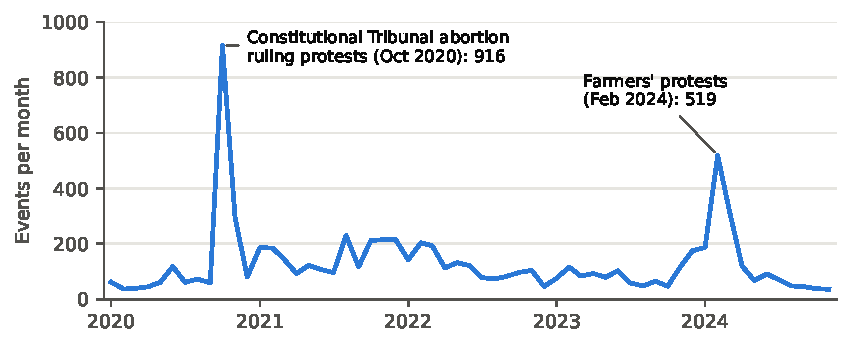
\includegraphics[width=\linewidth]{fig-monthly.pdf}
\caption{ACLED events per month in Poland, January 2020 to November 2024 (complete months).}
\label{fig:monthly}
\end{figure}

\subsection{Data licensing}
\label{sec:data-licence}

ACLED's terms permit the use of its data for research and the publication of derived, aggregated results with attribution, but not the redistribution of the original event records. The public repository therefore contains (i) the application code, (ii) the county-by-month counts used in the evaluation, which cannot be turned back into events, and (iii) a script that builds the application's event file from a user's own ACLED API access or from a CSV export from ACLED's website. Credentials are read from the environment and never stored.

%======================================================================
\section{Application design}
\label{sec:design}

\subsection{Principles}

Four principles guided the design.

\begin{description}[leftmargin=1.2em,style=nextline]
  \item[P1 Overview, filter, details on demand \cite{shneiderman1996}.] The map opens on the whole country with nearby events grouped; filters narrow the set; selecting a place shows the full record of each event.
  \item[P2 Places, not points.] Because most events share coordinates with others, selecting a location must open \emph{all} events at that location, not the one that happens to be drawn on top.
  \item[P3 A forecast must show its working.] Each county forecast is displayed with the three monthly counts it averages, the twelve-month history and the method's measured accuracy, including that of trivial baselines.
  \item[P4 Phones are a first-class target.] The same functions are available on a phone, where the map stays visible and the panel becomes a bottom sheet.
\end{description}

\subsection{Architecture}

Figure~\ref{fig:arch} shows the architecture. An ASP.NET Core 8 application loads the local ACLED extract once at start-up, skipping malformed records instead of failing, and keeps the events in memory. Three read-only endpoints serve the client: a compact list of all events for the map, filters and charts (date, position, type, sub-type, administrative units, interaction and fatalities; about 200\,kB compressed for 7{,}794 events); the full record of one event, requested only when it is opened; and the forecast for all counties with the backtest of the method. Narrative fields---notes, actors and sources---are therefore transferred only for the events a user actually reads. The forecast and its backtest are computed by the server from the same events the map shows, so the displayed numbers and the data cannot drift apart. The browser renders the map with the Google Maps JavaScript API, clusters markers with a supercluster-based clusterer and draws charts with Chart.js; both libraries are served from the application at fixed versions.

\begin{figure}[htbp]
\centering
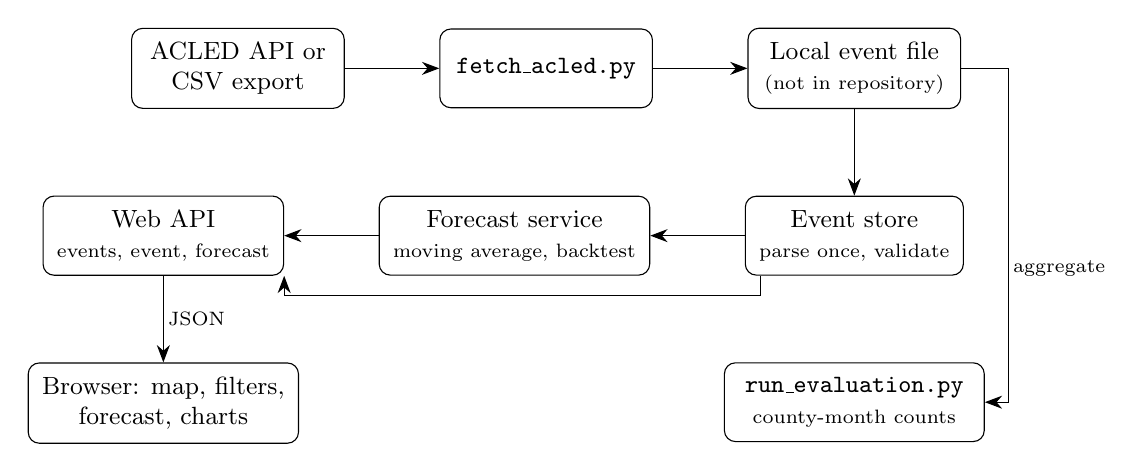
\begin{tikzpicture}[
    box/.style={draw, rounded corners, align=center, font=\small, inner sep=5pt, minimum width=2.7cm, minimum height=1.0cm},
    lbl/.style={font=\scriptsize, fill=white, inner sep=1.5pt},
    >={Stealth[length=2.2mm]}]
  \node[box] (acled) {ACLED API or\\ CSV export};
  \node[box, right=1.2cm of acled] (fetch) {\texttt{fetch\_acled.py}};
  \node[box, right=1.2cm of fetch] (file) {Local event file\\ \scriptsize(not in repository)};
  \node[box, below=1.1cm of file] (store) {Event store\\ \scriptsize parse once, validate};
  \node[box, left=1.2cm of store] (fc) {Forecast service\\ \scriptsize moving average, backtest};
  \node[box, left=1.2cm of fc] (api) {Web API\\ \scriptsize events, event, forecast};
  \node[box, below=1.1cm of api] (ui) {Browser: map, filters,\\ forecast, charts};
  \node[box, below=1.1cm of store, minimum width=3.3cm] (eval) {\texttt{run\_evaluation.py}\\ \scriptsize county-month counts};
  \draw[->] (acled) -- (fetch);
  \draw[->] (fetch) -- (file);
  \draw[->] (file) -- (store);
  \draw[->] (store) -- (fc);
  \draw[->] (fc) -- (api);
  \draw[->] (store.south west) ++(0.2,0) |- ++(0,-0.25) -| (api.south east);
  \draw[->] (api) -- node[lbl,right]{JSON} (ui);
  \draw[->] (file.east) -- ++(0.6,0) |- (eval.east) node[lbl,pos=0.3,right]{aggregate};
\end{tikzpicture}
\caption{Architecture. Raw events stay on the user's machine; only aggregated county-month counts are published with the evaluation.}
\label{fig:arch}
\end{figure}

\subsection{Interface}

The desktop layout places a panel with three views---\emph{Explore}, \emph{Forecast} and \emph{Insights}---beside the map (Figure~\ref{fig:overview}). \emph{Explore} offers filters by event type, sub-type, voivodeship and county (dependent lists with event counts), a period and the actors involved, together with a place search. Event markers use three colours---protests, riots and all other types---because a map of overlapping points can only keep a small number of categories distinguishable, also for readers with colour-vision deficiencies; groups of events are drawn as dark circles labelled with the number of events.

Selecting a group whose events share one location, or any marker, opens an event card listing the events at that place, newest first, with previous and next controls (Figure~\ref{fig:event}). The card shows the event type and sub-type, the date and place, ACLED's note, the actors, the interaction, fatalities, the location precision in plain words and the reporting source. This implements P2: in the Warsaw example the card offers all 1{,}132 events at the city-centre coordinate instead of a single marker that hides the others. Groups of events at one coordinate keep their count at every zoom level, so a stack is never mistaken for a single event. The same card can also be opened from the filter panel for the whole current selection (up to 2{,}000 events), which makes every record reachable with the keyboard alone and without the map.

\emph{Insights} shows four charts that follow the filters: events per month, event types, sub-event types and the ten counties with most events (Figure~\ref{fig:insights}). An incomplete final month is drawn dashed and labelled. \emph{Forecast} lists counties by their forecast for the next month (Figure~\ref{fig:forecast}). Each entry shows the forecast, the three months it averages, a twelve-month sparkline, the events already recorded in the forecast month and the expected number of events by sub-type; choosing a county filters and zooms the map to it. An expandable section reports the backtest of the moving average next to the naive and always-zero baselines (\S\ref{sec:res-accuracy}).

On phones the map fills the screen and the panel becomes a bottom sheet that shows the view tabs and a one-line summary when collapsed (Figure~\ref{fig:phone}). Opening an event collapses the sheet so that the card and the map remain visible together. A light and a dark theme are available; the dark theme follows the operating-system setting unless the user chooses otherwise, uses a neutral dark basemap so that the three data colours remain the strongest marks, and switches the data colours to steps validated for contrast and colour-vision separation on the dark background.

\begin{figure}[htbp]
\centering
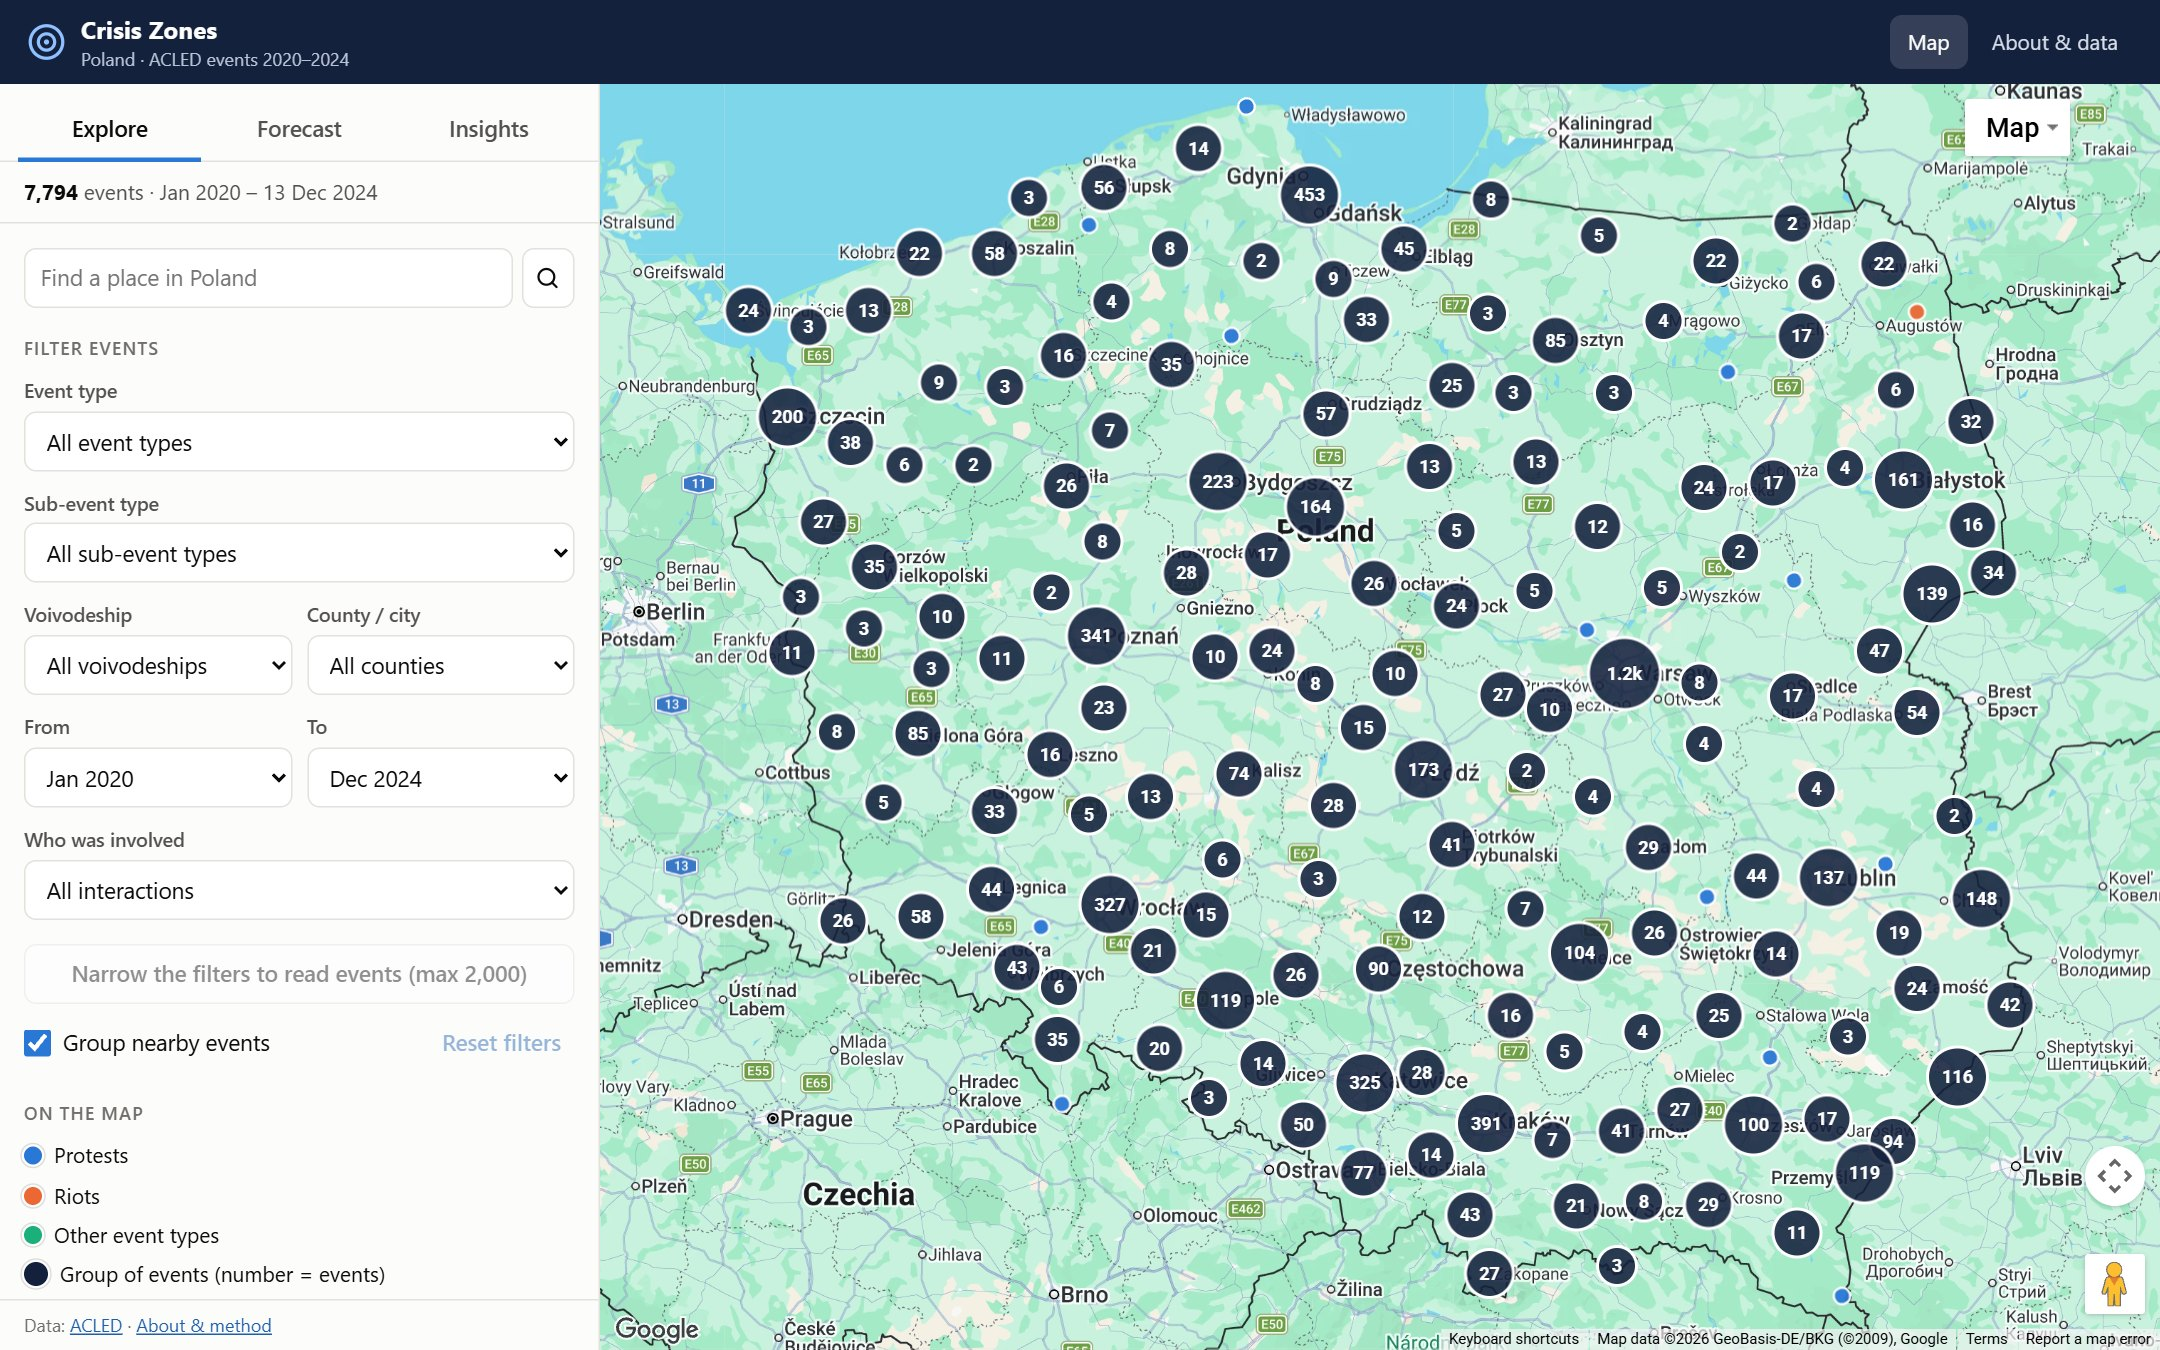
\includegraphics[width=\linewidth]{app-overview.jpg}
\caption{Overview: all 7{,}794 events grouped by proximity, with the \emph{Explore} filters.}
\label{fig:overview}
\end{figure}

\begin{figure}[htbp]
\centering
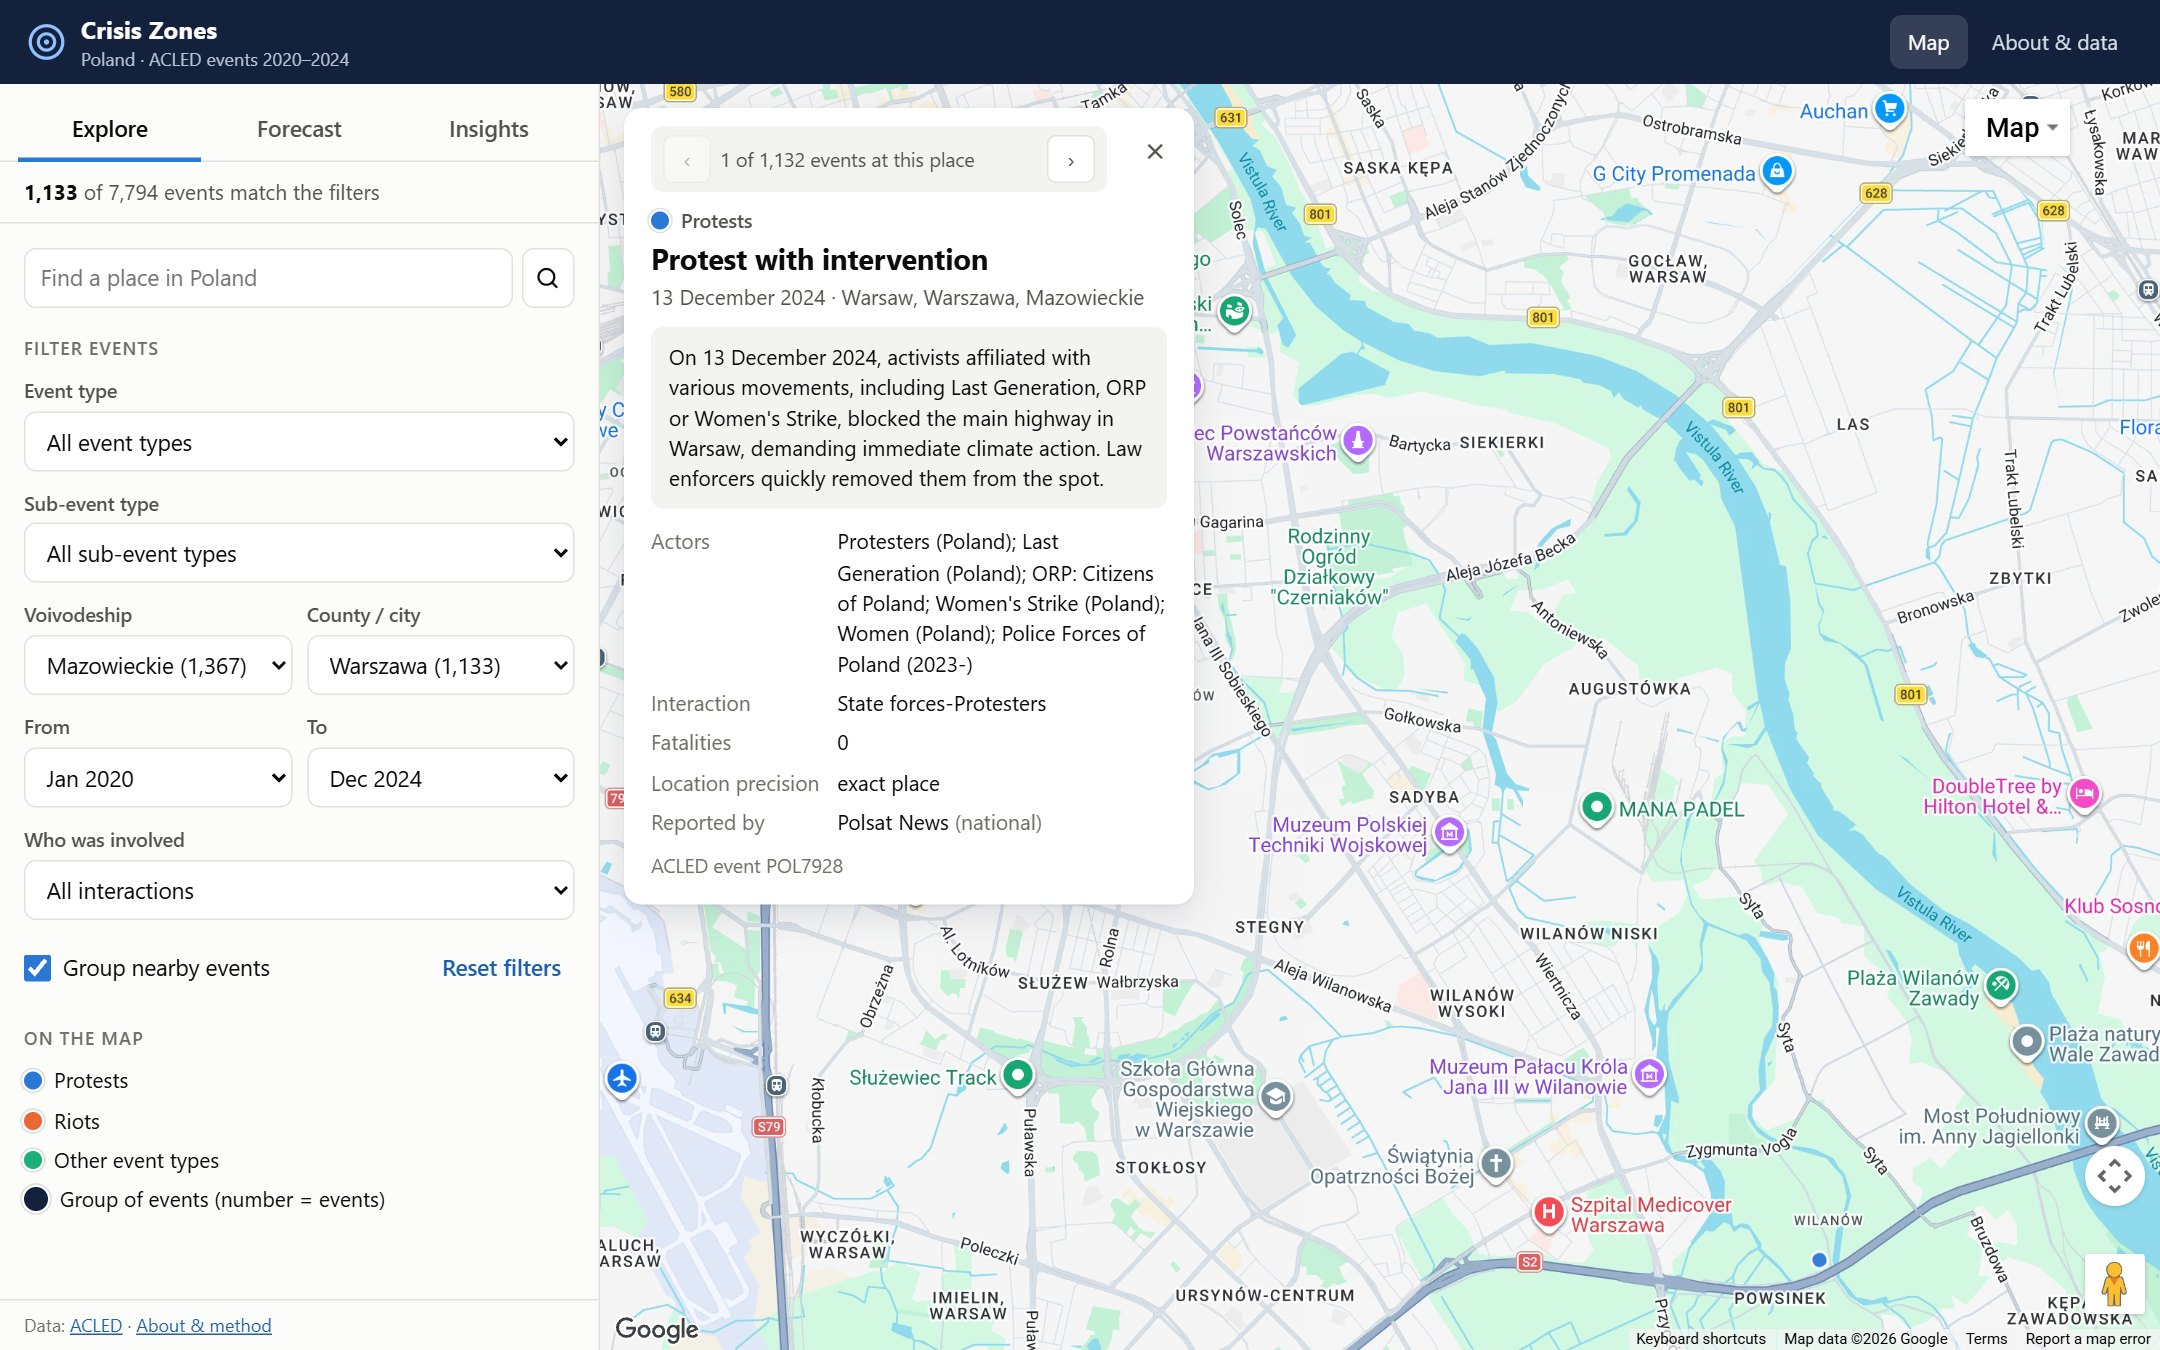
\includegraphics[width=\linewidth]{app-event.jpg}
\caption{Place-level event browsing in Warsaw. The card offers all events at the selected coordinate, newest first, with ACLED's note, actors and source.}
\label{fig:event}
\end{figure}

\begin{figure}[htbp]
\centering
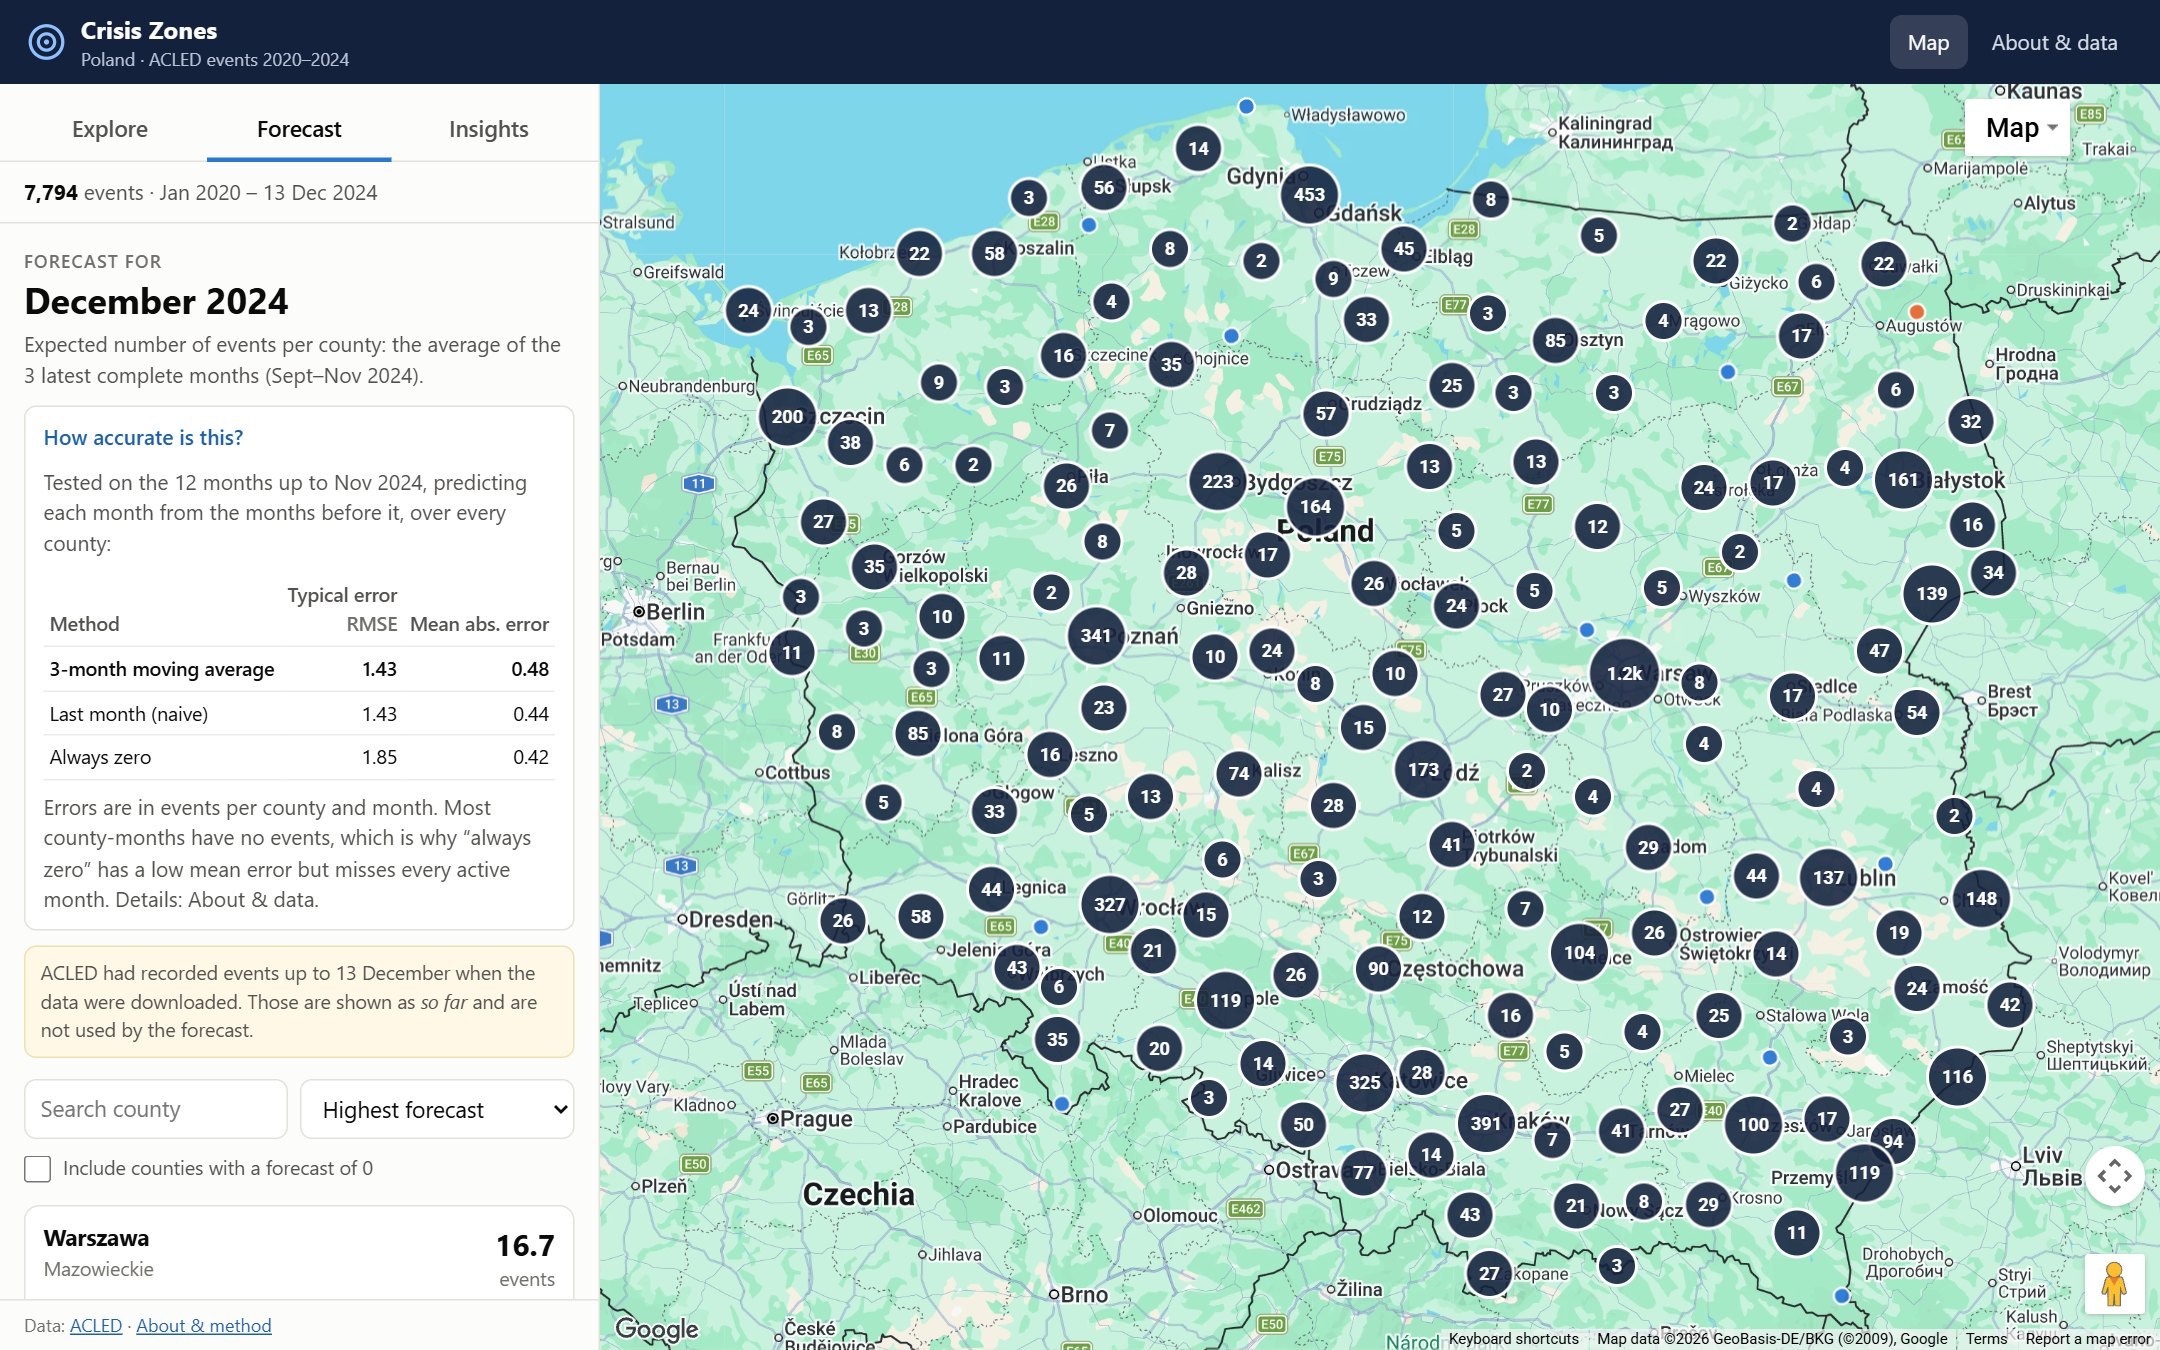
\includegraphics[width=\linewidth]{app-forecast.jpg}
\caption{Forecast view with the backtest of the method expanded. Every county entry shows the three months its forecast averages.}
\label{fig:forecast}
\end{figure}

\begin{figure}[htbp]
\centering
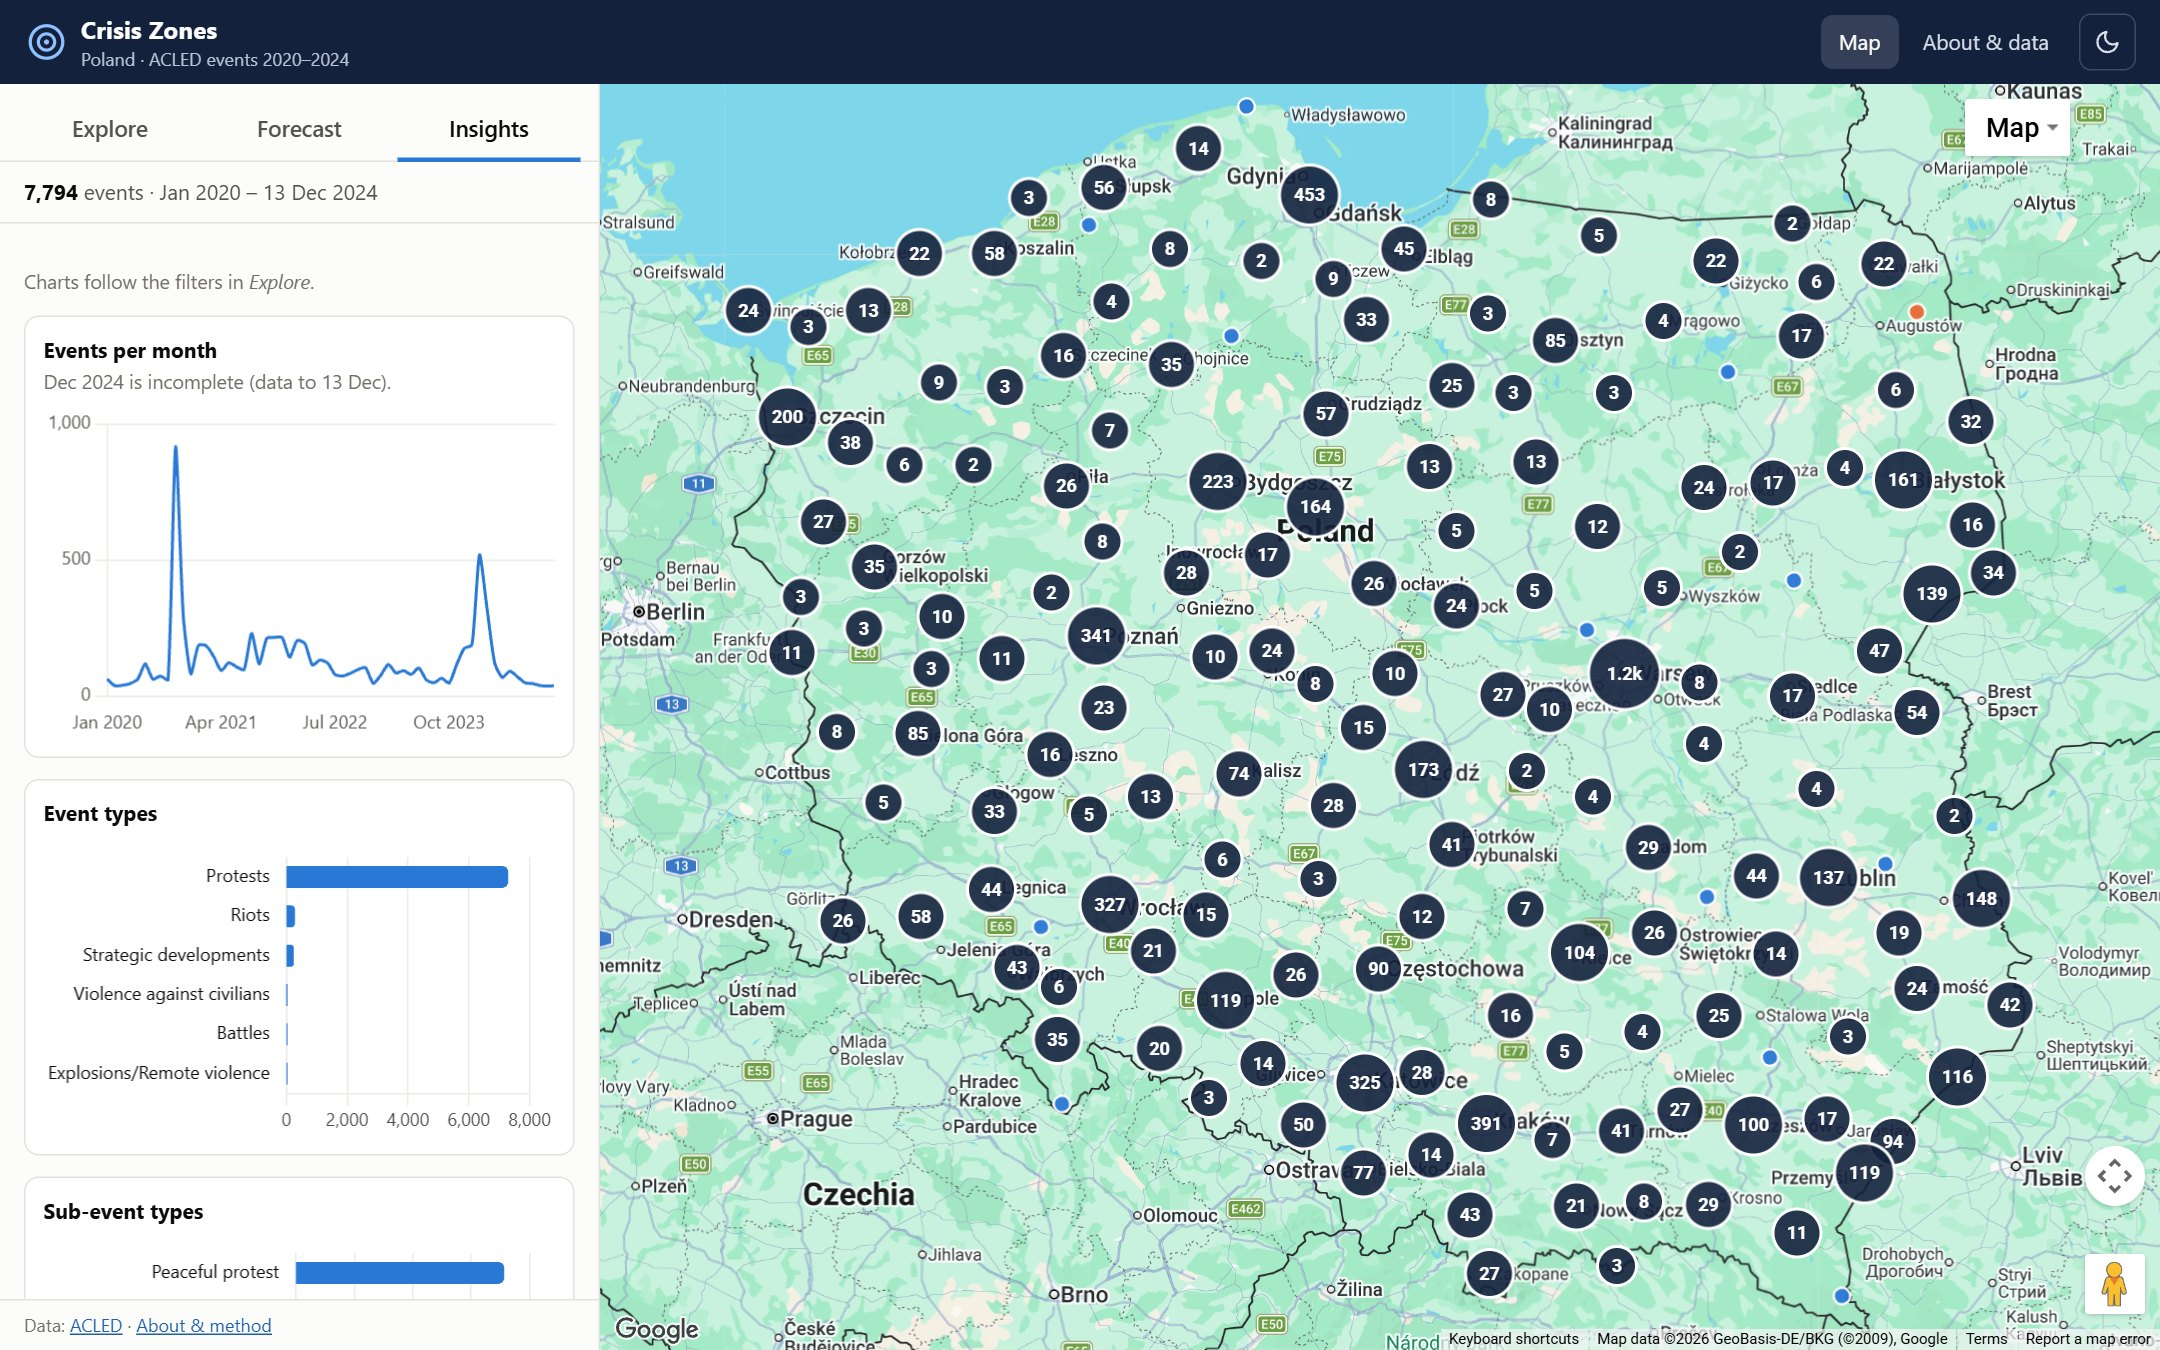
\includegraphics[width=\linewidth]{app-insights.jpg}
\caption{Insights: charts that follow the current filters.}
\label{fig:insights}
\end{figure}

\begin{figure}[htbp]
\centering
\begin{subfigure}{0.31\linewidth}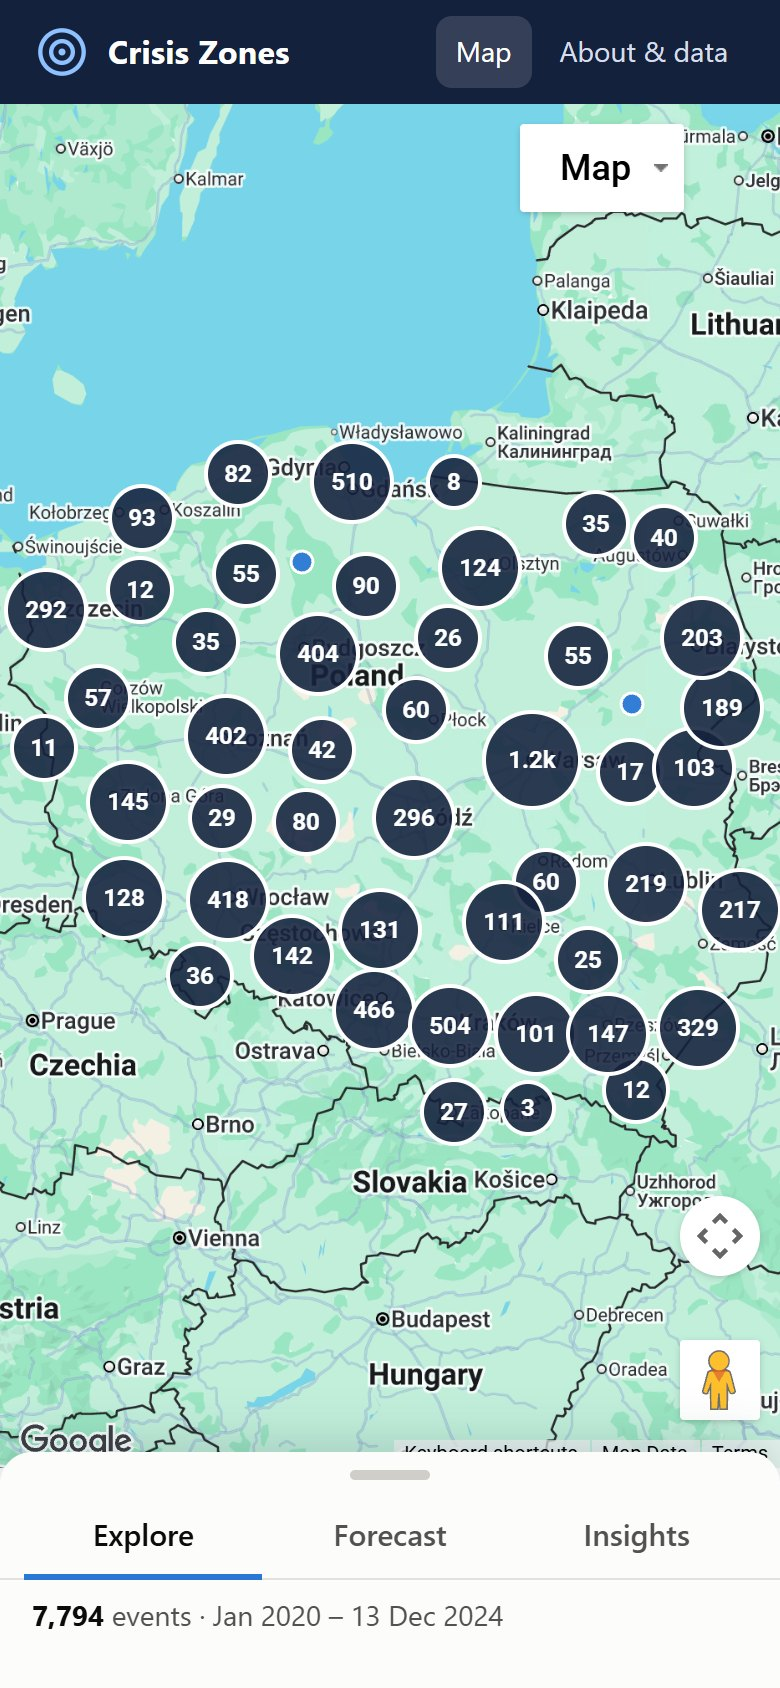
\includegraphics[width=\linewidth]{phone-home.jpg}\caption{Overview}\end{subfigure}\hfill
\begin{subfigure}{0.31\linewidth}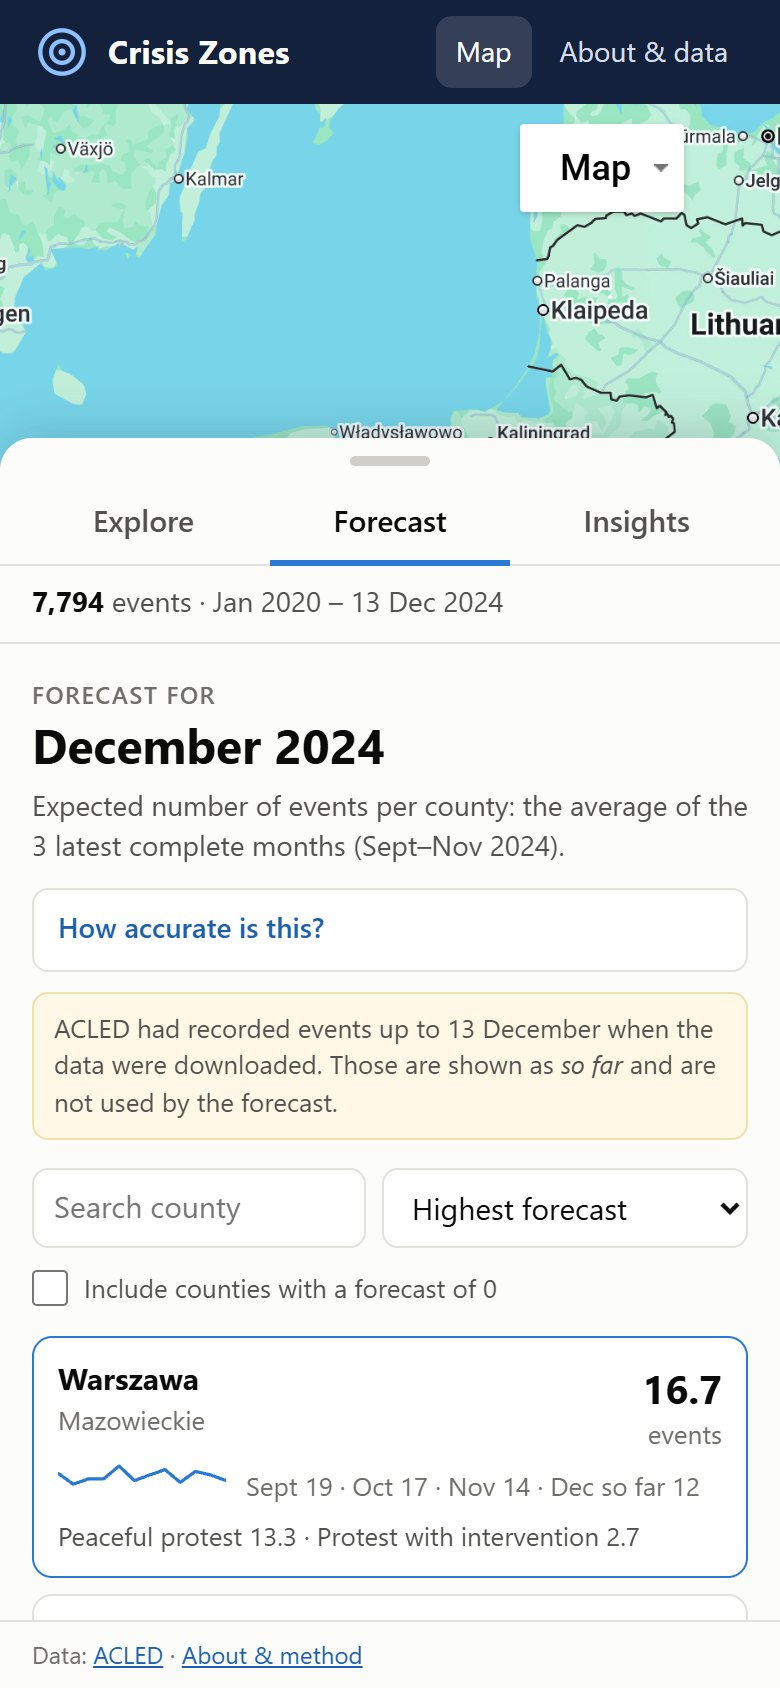
\includegraphics[width=\linewidth]{phone-forecast.jpg}\caption{Forecast sheet}\end{subfigure}\hfill
\begin{subfigure}{0.31\linewidth}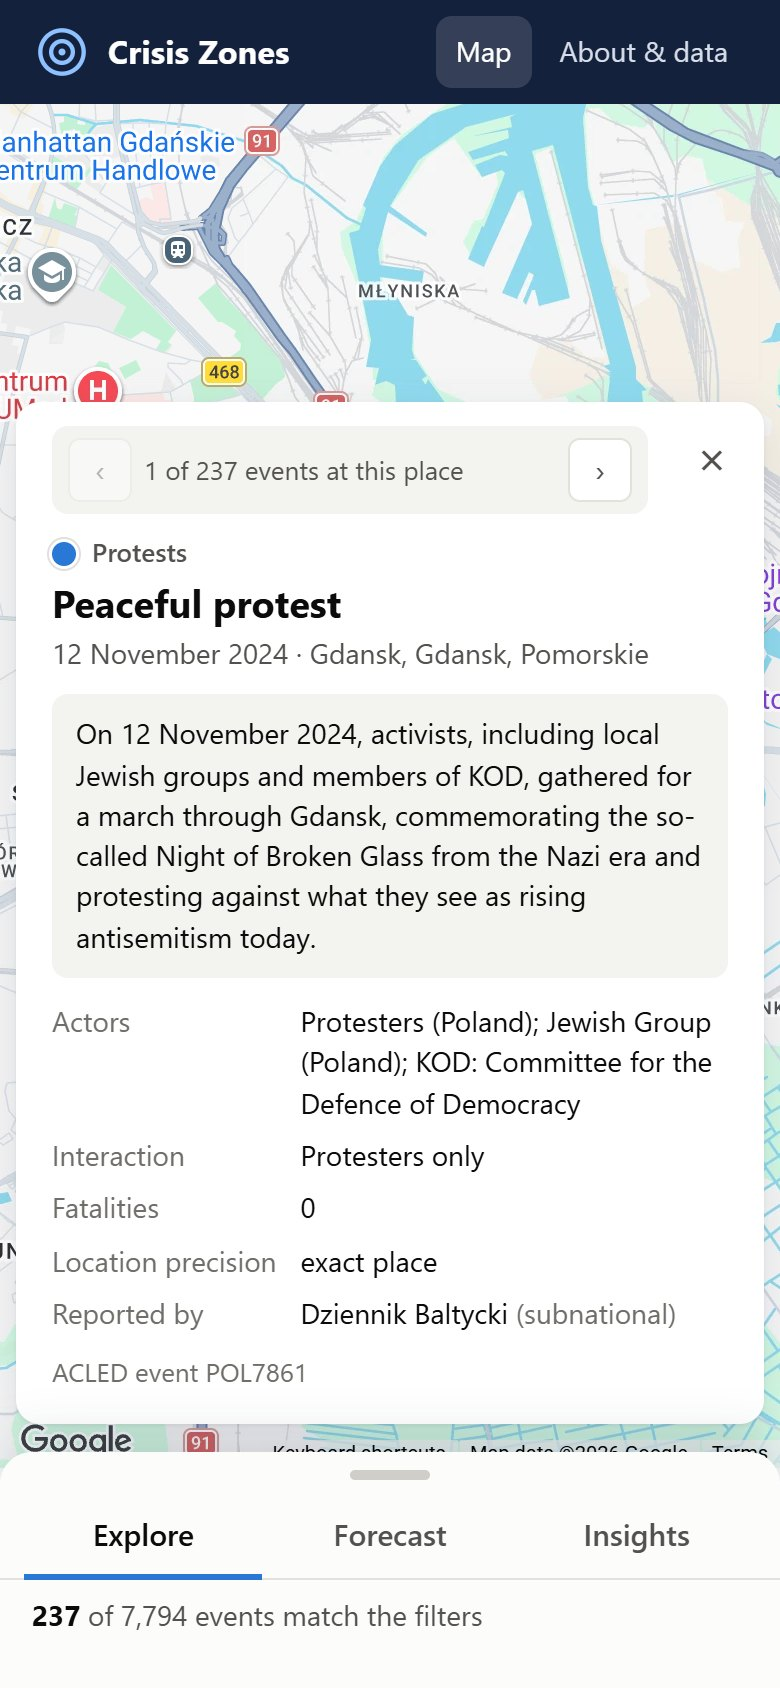
\includegraphics[width=\linewidth]{phone-event.jpg}\caption{Event at a place}\end{subfigure}
\caption{Phone layout (390\,px wide). The panel becomes a bottom sheet; the map stays visible.}
\label{fig:phone}
\end{figure}

\subsection{Robustness, security and privacy}

The event loader validates every record (identifier, date, coordinates within valid ranges and not at 0,\,0) and counts rejected records instead of stopping; dates in ISO form and as GIS epoch milliseconds are both accepted. If the event file is missing, the API answers with a clear message and the page still loads. All text from the data is inserted into the page as text, never as markup, so a note cannot inject script; in addition, a content security policy allows scripts only from the application and Google Maps. Responses carry standard protective headers, error responses are never cached, the raw event file is outside the web root, and the Google Maps key is read from a local configuration file excluded from version control. Event dates are calendar dates and are displayed independently of the viewer's time zone. The application has no accounts, sets no cookies and stores nothing about its users. Twenty-eight automated tests cover parsing and validation, the completeness rule, the moving average and backtest, and the API behaviour; six further tests cover the download script, including ACLED exports that write dates in words.

%======================================================================
\section{Forecast evaluation}
\label{sec:eval}

\subsection{Task and data}

The task is to predict the number of ACLED events in each county in the next calendar month. The evaluation uses the 59 complete months and all 341 counties that recorded at least one event, giving 20{,}119 county-months; 85.2\% of them have no events. Months without events are included as zeros.

\subsection{Methods}

Eight methods are compared. Let $y_{c,t}$ be the count for county $c$ in month $t$.
\begin{itemize}
  \item \emph{Always zero}: $\hat y_{c,t}=0$.
  \item \emph{Last month (naive)}: $\hat y_{c,t}=y_{c,t-1}$.
  \item \emph{Same month last year}: $\hat y_{c,t}=y_{c,t-12}$.
  \item \emph{Historical mean}: the mean of all earlier months of the county.
  \item \emph{3-month moving average} (the method shown in the application): $\hat y_{c,t}=\tfrac13(y_{c,t-1}+y_{c,t-2}+y_{c,t-3})$.
  \item \emph{6-month moving average}.
  \item \emph{Poisson GLM}: a Poisson regression on $\log(1+y_{c,t-k})$, $k=1,2,3$.
  \item \emph{Random Forest} \cite{breiman2001}: 300 trees of depth at most 8, on a county identifier, the calendar month and lags one to three.
\end{itemize}
The two learned models are fitted once on all months before the test window \cite{pedregosa2011}.

\subsection{Protocol}

The protocol is a rolling one-step-ahead evaluation. Every month in the test window is predicted from the observed months before it, and all methods receive the same history. The primary test window is the last 12 complete months (December 2023 to November 2024; 4{,}092 county-months, 619 of them with events); windows of 6 and 24 months are reported as sensitivity checks.

\subsection{Metrics and uncertainty}

Four measures are reported: MAE and RMSE over all county-months, MAE over the county-months with at least one event, and the mean Poisson deviance (not defined for a forecast of exactly zero). RMSE is used as the primary measure because it is minimised by the expected count, which is what the application displays \cite{gneiting2011}. Differences in RMSE are given with 95\% intervals from a bootstrap that resamples counties (2{,}000 resamples), which respects the dependence of months within a county.

\subsection{A second evaluation design}

To answer RQ4, the moving average, the naive method and the Random Forest are also scored under an \emph{events-only} design that reflects choices common in quick evaluations: only county-months with at least one event are kept; the moving average and naive forecasts look up earlier months in the training period only, so inside the test window they often find nothing and predict zero; and the Random Forest's lags are the previous rows \emph{with events}, taken from the test period itself. The two designs therefore differ in which rows are scored and in the information each method receives.

%======================================================================
\section{Results}
\label{sec:results}

\subsection{Spatial and temporal structure (RQ2)}
\label{sec:res-patterns}

Activity is concentrated. Warsaw alone accounts for 14.5\% of events (1{,}133), and the five largest cities---Warsaw, Kraków, Poznań, Wrocław and Gdańsk---for 29.1\%; the ten most active counties for 39.7\%. The median county recorded 8 events in five years, and 131 counties recorded five or fewer. In time, the record combines a slowly varying level with short national waves (Figure~\ref{fig:monthly}) that start abruptly in response to political events. For forecasting, this means that most county-months are zero, that the few active counties dominate any squared-error measure, and that the largest errors will occur at the start of waves, which no method based on recent counts can anticipate.

\subsection{Forecast accuracy (RQ3)}
\label{sec:res-accuracy}

Table~\ref{tab:accuracy} and Figure~\ref{fig:rmse} report the primary window. Ordered by RMSE, the Random Forest is first (1.35), followed by the 3-month moving average (1.43) and the naive forecast (1.43); always predicting zero is last (1.85). Ordered by MAE, the order reverses: always zero has the lowest MAE (0.42), because it is right in 85\% of county-months, while missing every active month by 2.8 events on average. The Poisson deviance favours the two count models, whose forecasts are never exactly zero.

\begin{table}[htbp]
\centering
\small
\caption{Accuracy on December 2023 to November 2024 (4{,}092 county-months; 619 with events). Sorted by RMSE; lower is better.}
\label{tab:accuracy}
\begin{tabular}{lrrrr}
\toprule
Method & MAE & RMSE & MAE, months with events & Poisson deviance \\
\midrule
Random Forest (lags + month) & 0.504 & 1.351 & 1.915 & 1.354 \\
3-month moving average & 0.483 & 1.426 & 1.914 & 3.608 \\
Last month (naive) & 0.441 & 1.434 & 1.932 & 4.402 \\
Poisson GLM (lags) & 0.512 & 1.462 & 2.001 & 1.209 \\
6-month moving average & 0.525 & 1.523 & 1.938 & 3.375 \\
Historical mean & 0.510 & 1.541 & 2.056 & 1.641 \\
Same month last year & 0.434 & 1.726 & 2.204 & 7.258 \\
Always zero & 0.419 & 1.852 & 2.771 & -- \\
\bottomrule
\end{tabular}
\end{table}

\begin{figure}[htbp]
\centering
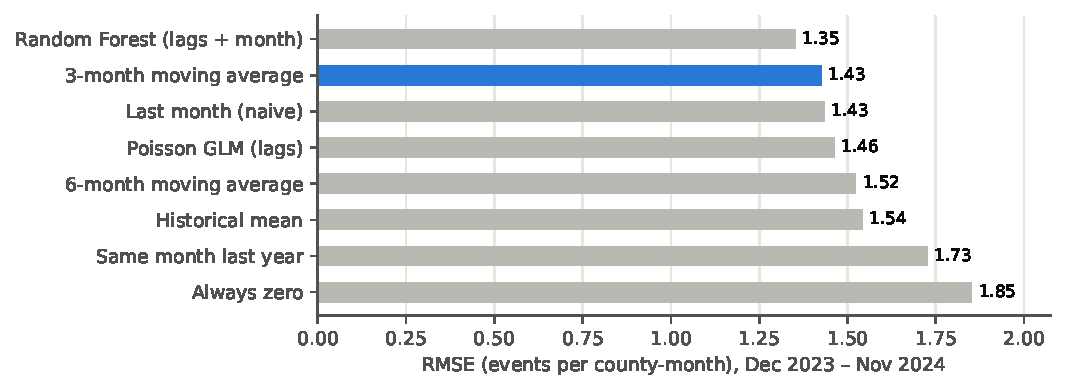
\includegraphics[width=\linewidth]{fig-rmse.pdf}
\caption{RMSE by method on the primary test window. The method shown in the application is highlighted.}
\label{fig:rmse}
\end{figure}

The differences among the leading methods are small relative to their uncertainty. The bootstrap difference in RMSE between the moving average and the Random Forest is $+0.074$ (95\% interval $-0.082$ to $+0.234$); between the moving average and the naive forecast $-0.008$ ($-0.178$ to $+0.169$); and between the moving average and the Poisson GLM $-0.037$ ($-0.129$ to $+0.069$). None of the intervals excludes zero.

The ranking also changes with the window. On the last 6 months, a quiet period with 135 active county-months, the Poisson GLM has the lowest RMSE (0.66), followed by the moving average (0.72) and the Random Forest (0.75). On the last 24 months the Random Forest (1.17), the moving average (1.18) and the Poisson GLM (1.20) are within 0.03 of each other. Split by county activity, the Random Forest gains most in counties with a moderate level of events (0.5 to 2 per month: RMSE 2.87 against 3.17), whereas in the most active counties (more than 2 per month) the moving average is marginally better (2.86 against 2.88).

The backtest computed by the application matches the evaluation script for the three methods it reports to three decimals (moving average 0.483 and 1.426, naive 0.441 and 1.434, always zero 0.419 and 1.852, as MAE and RMSE), which confirms that the displayed accuracy describes the displayed forecast.

\subsection{Effect of the evaluation design (RQ4)}
\label{sec:res-protocol}

Figure~\ref{fig:protocol} compares the two designs on the same test months. Under the events-only design, the Random Forest's MAE is 1.68 against 2.42 for the moving average and 2.60 for the naive forecast: an apparent 30\% advantage. When the same methods are scored on the same county-months with the same information, the three MAEs are 1.92, 1.91 and 1.93. The apparent advantage comes from the design: the baselines were denied the months they are defined on, while the learned model's lags came from the test period. Dropping months without events changes the picture further, because it removes exactly the cases in which persistence forecasts are most often right.

\begin{figure}[htbp]
\centering
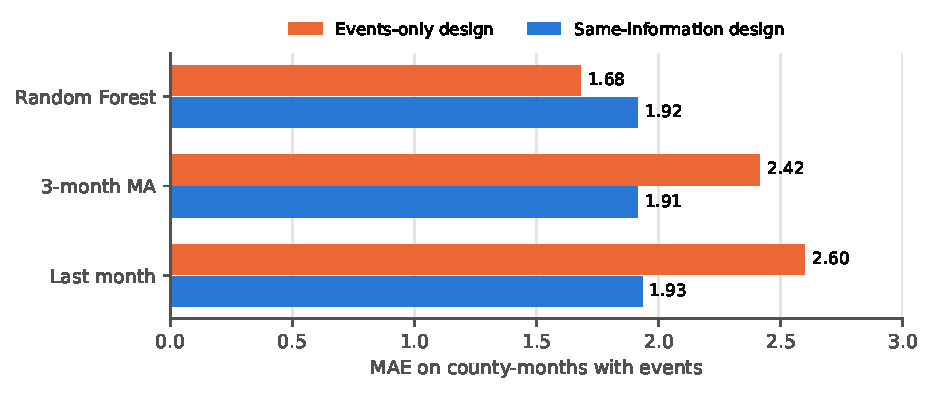
\includegraphics[width=\linewidth]{fig-protocol.pdf}
\caption{The same three methods under two evaluation designs, on the county-months with events in the primary test window.}
\label{fig:protocol}
\end{figure}

\subsection{Application (RQ1)}
\label{sec:res-app}

The application meets the four principles. The national overview, filtering and details-on-demand sequence works on desktop and on phones from 360\,px wide, with the map remaining visible in every state. Treating places as the unit of selection makes events reachable that a point map hides: at 95.5\% of events sharing coordinates, a conventional marker-and-popup design would show one event per place and hide the remaining 6{,}996. Every forecast value can be recomputed by hand from the three numbers shown beside it, and the panel states the method's accuracy against the baselines, including the one that predicts no activity. Loading the event list once and fetching the narrative record on demand keeps the initial transfer to about 200\,kB.

%======================================================================
\section{Discussion}
\label{sec:discussion}

\subsection{Which forecast to show}

On accuracy alone, no method dominates. The Random Forest has the lowest RMSE on the primary and the longest window but not on the shortest, its advantage is within sampling uncertainty, and it gains mainly in moderately active counties. The moving average is within 0.08 RMSE of it, can be checked by anyone from three numbers, and behaves predictably at the start and end of protest waves: it rises and falls with a lag of about one month. For a public, explanatory interface the moving average is therefore the better default. A learned model would be worth displaying if it were shown to anticipate the onset of waves, which none of the methods here do, or if it provided calibrated uncertainty; both are directions for future work.

\subsection{Reporting accuracy with its protocol}

The comparison of designs shows that a single accuracy number is not interpretable without the protocol behind it. Three choices proved decisive: whether months without events are counted, whether all methods receive the same information, and which metric is used. With sparse counts, MAE favours forecasting no activity and should not be reported alone. The application reports RMSE and MAE for its method next to a naive and an always-zero baseline; the evaluation adds the Poisson deviance and bootstrap intervals. This practice---always showing trivial baselines and the uncertainty of differences---is cheap and guards against overstated claims of predictive skill \cite{ward2010,hegre2022}.

\subsection{Implications for GEOINT and civil-protection use}

For analysts, the main value of the application is speed of orientation: from the national picture to the events behind a county in a few interactions, with the source and the narrative note of each event at hand. The forecast panel adds a short-term expectation per county that is honest about its limits. It is not an early-warning system: it extrapolates recent reporting and cannot anticipate a court ruling, an election or a policy decision that starts a new wave. Its appropriate use is as a baseline expectation against which unusual activity becomes visible.

\subsection{Limitations}

ACLED records reported events, and reporting is uneven across places and time \cite{weidmann2016,raleigh2023}; quieter counties may be under-recorded rather than quiet. Counties differ greatly in population and size, and the analysis does not normalise counts. Geocoding to place centres means the map cannot show where within a city an event took place. The evaluation covers one country and five years, with two dominant protest waves; results for countries with armed conflict may differ. ACLED revises records over time, so a new download can differ slightly from the extract used here; the published county-month counts make the evaluation reproducible regardless. Finally, the learned models were not tuned extensively; a tuned model might gain more, but the evaluation design, not tuning, was the larger source of difference in this study.

\subsection{Ethics}

The application displays ACLED's published summaries of public events. Narrative notes can name groups and, occasionally, people; the application shows them only one event at a time, adds nothing to them and does not link them to other data. The forecast is labelled as an expectation from recent counts, not as an assessment of risk or of any group's intentions.

%======================================================================
\section{Conclusion}
\label{sec:conclusion}

\appname{} shows that an event dataset of several thousand records can be explored from national overview to individual event on desktop and phone, provided the interface treats places rather than points as the unit of selection: in the Polish ACLED record, 95.5\% of events share a location with others. For next-month county forecasts, a three-month moving average is statistically indistinguishable from the best of seven alternatives, including a Random Forest, and has the advantage that every value can be checked. How a forecast is evaluated changed the conclusions more than which forecast was used: the same Random Forest appears 30\% more accurate than the moving average under one plausible design and equal to it under a design in which all methods see the same information. Forecast panels in GEOINT applications should therefore report accuracy together with the protocol, the metric and trivial baselines.

\section*{Data and code availability}

Source code, tests, the evaluation script, the aggregated county-month counts and this paper: \url{\repourl}~\archivedoi. ACLED event data must be obtained from ACLED (\url{https://acleddata.com}); the repository includes a script that builds the application's event file from an ACLED account. Data attribution: Armed Conflict Location \& Event Data (ACLED), \url{https://acleddata.com}.

%======================================================================
\begin{thebibliography}{99}
\small

\bibitem{acled2024} ACLED, \emph{ACLED Codebook}. Armed Conflict Location \& Event Data, 2024. \url{https://acleddata.com}

\bibitem{bergmeir2012} C.~Bergmeir and J.~M. Benítez, ``On the use of cross-validation for time series predictor evaluation,'' \emph{Information Sciences}, vol.~191, pp.~192--213, 2012.

\bibitem{bowlsby2020} D.~Bowlsby, E.~Chenoweth, C.~Hendrix, and J.~D. Moyer, ``The future is a moving target: Predicting political instability,'' \emph{British Journal of Political Science}, vol.~50, no.~4, pp.~1405--1417, 2020.

\bibitem{breiman2001} L.~Breiman, ``Random forests,'' \emph{Machine Learning}, vol.~45, no.~1, pp.~5--32, 2001.

\bibitem{czado2009} C.~Czado, T.~Gneiting, and L.~Held, ``Predictive model assessment for count data,'' \emph{Biometrics}, vol.~65, no.~4, pp.~1254--1261, 2009.

\bibitem{diebold1995} F.~X. Diebold and R.~S. Mariano, ``Comparing predictive accuracy,'' \emph{Journal of Business \& Economic Statistics}, vol.~13, no.~3, pp.~253--263, 1995.

\bibitem{gneiting2011} T.~Gneiting, ``Making and evaluating point forecasts,'' \emph{Journal of the American Statistical Association}, vol.~106, no.~494, pp.~746--762, 2011.

\bibitem{hegre2019} H.~Hegre \emph{et al.}, ``ViEWS: A political violence early-warning system,'' \emph{Journal of Peace Research}, vol.~56, no.~2, pp.~155--174, 2019.

\bibitem{hegre2021} H.~Hegre \emph{et al.}, ``ViEWS2020: Revising and evaluating the ViEWS political violence early-warning system,'' \emph{Journal of Peace Research}, vol.~58, no.~3, pp.~599--611, 2021.

\bibitem{hegre2022} H.~Hegre, P.~Vesco, and M.~Colaresi, ``Lessons from an escalation prediction competition,'' \emph{International Interactions}, vol.~48, no.~4, pp.~521--554, 2022.

\bibitem{hyndman2006} R.~J. Hyndman and A.~B. Koehler, ``Another look at measures of forecast accuracy,'' \emph{International Journal of Forecasting}, vol.~22, no.~4, pp.~679--688, 2006.

\bibitem{kapoor2023} S.~Kapoor and A.~Narayanan, ``Leakage and the reproducibility crisis in machine-learning-based science,'' \emph{Patterns}, vol.~4, no.~9, 100804, 2023.

\bibitem{nga2018} National Geospatial-Intelligence Agency, \emph{Geospatial Intelligence (GEOINT) Basic Doctrine}, Publication 1-0. Springfield, VA: NGA, 2018.

\bibitem{pedregosa2011} F.~Pedregosa \emph{et al.}, ``Scikit-learn: Machine learning in Python,'' \emph{Journal of Machine Learning Research}, vol.~12, pp.~2825--2830, 2011.

\bibitem{raleigh2010} C.~Raleigh, A.~Linke, H.~Hegre, and J.~Karlsen, ``Introducing ACLED: An Armed Conflict Location and Event Dataset,'' \emph{Journal of Peace Research}, vol.~47, no.~5, pp.~651--660, 2010.

\bibitem{raleigh2023} C.~Raleigh, R.~Kishi, and A.~Linke, ``Political instability patterns are obscured by conflict dataset scope conditions, sources, and coding choices,'' \emph{Humanities and Social Sciences Communications}, vol.~10, 74, 2023.

\bibitem{repo} S.~Arzimanli, \emph{Crisis Zones: source code, evaluation and aggregated data}, version 1.1.0, 2026. \url{\repourl}, doi:10.5281/zenodo.24417729

\bibitem{shneiderman1996} B.~Shneiderman, ``The eyes have it: A task by data type taxonomy for information visualizations,'' in \emph{Proc. IEEE Symposium on Visual Languages}, 1996, pp.~336--343.

\bibitem{tashman2000} L.~J. Tashman, ``Out-of-sample tests of forecasting accuracy: An analysis and review,'' \emph{International Journal of Forecasting}, vol.~16, no.~4, pp.~437--450, 2000.

\bibitem{vesco2022} P.~Vesco \emph{et al.}, ``United they stand: Findings from an escalation prediction competition,'' \emph{International Interactions}, vol.~48, no.~4, pp.~860--896, 2022.

\bibitem{ward2010} M.~D. Ward, B.~D. Greenhill, and K.~M. Bakke, ``The perils of policy by p-value: Predicting civil conflicts,'' \emph{Journal of Peace Research}, vol.~47, no.~4, pp.~363--375, 2010.

\bibitem{weidmann2016} N.~B. Weidmann, ``A closer look at reporting bias in conflict event data,'' \emph{American Journal of Political Science}, vol.~60, no.~1, pp.~206--218, 2016.

\end{thebibliography}

\end{document}
